\documentclass[11pt,a4paper]{article}

\usepackage[utf8]{inputenc}
\usepackage[cyr]{aeguill}
\usepackage[francais]{babel}

% Les packages
%\usepackage[french]{babel}
\usepackage{fancybox}
\usepackage{graphics}
\usepackage{color}
\usepackage{latexsym}
\usepackage{amsmath,amsthm,amssymb}
\usepackage[plain]{fullpage} 
\usepackage{verbatim}
\usepackage{times,epsfig}
\usepackage{listings}
\usepackage{multirow}
\usepackage{amsmath,amsthm,amssymb,amscd,txfonts,bbm} % RAJOUT ICI !!!
\usepackage{graphics,epsfig} % RAJOUT ICI !!!
%\usepackage{algorithmic}
\usepackage[final]{pdfpages} 
\usepackage{fancyvrb}
\usepackage{enumerate}
\usepackage{listingsutf8}
\usepackage{comment}
\usepackage{minted}

% small et verbatim: to be coherent with \file
\newenvironment{smallverbatim}%
{\endgraf\small\verbatim}{\endverbatim}

\newenvironment{qv}
{\quote\Verbatim}
{\endquote\endVerbatim}

\usepackage{lastpage}

\newcommand{\terme}[1]{\texttt{#1}}
\newcommand{\termSet}[1]{\{\texttt{#1}\}}
\newcommand{\guill}[1]{<<\,#1\,>>}
% Macro pour l'inclusion de figure  
\newcommand{\fig}[2]{%
  \begin{figure*}[hbt]
   \begin{center}
      \includegraphics[width=6cm]{#1}
  \caption{\label{#1}  #2}
  \end{center}
 \end{figure*}
}
\newcommand{\figTex}[2]{%
  \begin{figure*}[hbt]
 \centerline{\input{#1.pstex_t}}
  \caption{\label{#1}  #2}
 \end{figure*}
}

% Macro commentaires
\definecolor{turquoise}{rgb}{0.20 ,0.60, 0.60}
\definecolor{vert}{rgb}{0.40,  0.60 ,0.00}
\definecolor{violet}{rgb}{0.80 , 0.00 , 0.80}
\definecolor{bleu}{rgb}{0.20,  0.20,  0.80}
\definecolor{rose}{rgb}{1.00,  0.20,  0.40}

\lstset{basicstyle=\footnotesize,showstringspaces=false,language=XML,breaklines=false,columns=fullflexible,frame=shadowbox, captionpos=b}

\newenvironment{solution}[0]{
~\\ \color{red} \textbf{Solution : }\color{black}}{%
}
%\excludecomment{solution}


\parindent=0pt           
                             
\usepackage{url}

\newtheorem{Exercice}{Definition}


\begin{document}

\title{Sujet d'examen UE NFE204 - Session 1}
\author{Année universitaire 2017-2018}
\date{Examen première session: 6 février 2018}

\maketitle

\begin{center}
{\bf \Large Consignes}\\
\begin{tabular}{| p{15cm} |}
\hline
Dur\'ee de l'examen : 3h00; Documents non autoris\'es;  Calculatrice autoris\'ee\\

Les exercices sont indépendants les uns des autres. Merci de soigner votre écriture.\\
Ce sujet contient \pageref{LastPage} pages.\\

\textit{Important}\,: nous n'évaluons pas les réponses par la syntaxe. Ne vous
inquiétez pas d'utiliser un point-virgule à la place d'un point d'exclamation ou
autres détails mineurs
\\
\hline
\end{tabular}
\end{center}

\emph{L'ensemble de l'examen doit vous permettre de montrer que vous avez assimilé les principales notions vues
en cours et en TP et que vous savez les mettre en application et les expliquer. La clarté, la concision,
la précision des réponses sera donc appréciée.}

\section*{Première partie : modélisation NoSQL (7 pts)}

Pour cette partie, nous allons nous pencher sur le petit tutoriel proposé par la documentation en ligne de
Cassandra, et consacré à la modélisation des données dans un contexte BigData. L'application (très simplifiée)
est un service de musique en ligne, avec le modèle de données de la figure~\ref{fig:musicservice}.

\begin{figure}[ht]
\centering
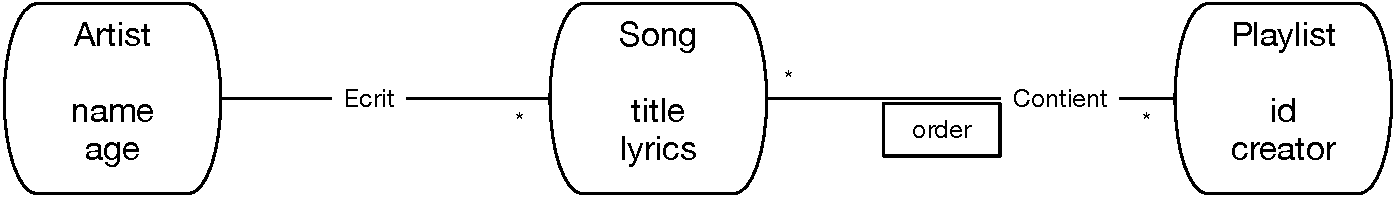
\includegraphics[width=0.8\textwidth]{../../../supports/figures/musicservice.pdf}
\caption{Modélisation d'un service de musique en ligne\label{fig:musicservice}}
\end{figure}

On a donc des chansons, chacune écrite par un artiste, et des \textit{playlists}, qui consistent
en une liste ordonnée de chansons.

\begin{enumerate}
  \item Commencer par proposer le schéma relationnel correspondant à ce modèle. Il est sans
      dout nécessaire d'ajouter des identifiants. Donnez les commandes SQL de création des tables. (1 pt).
   
   \item Le tutoriel Cassandra nous explique qu'il faut concevoir le schéma Cassandra en fonction
   des \textit{Access patterns}, autrement dit des requêtes que l'on s'attend à devoir effectuer. Voici
   les trois \textit{access patterns} envisagés:
   \begin{enumerate}
      \item \textit{Find all song titles}
      \item \textit{Find all songs titles of a particular playlist}
   \end{enumerate}
   
   Lesquels  de ces \textit{access patterns} posent potentiellement problème avec un système relationnel
   dans un contexte \textit{BigData} et pourquoi ? Vous pouvez donner les requêtes SQL correspondantes
   pour clarifier votre réponse (1 pt).
   
   \item Le tutoriel Cassandra nous propose alors de créer une unique table Cassandra suivante
   
\begin{minted}[frame=leftline,
               baselinestretch=.9,
               fontsize=\small,
               framesep=2mm]{sql}
CREATE TABLE playlists (
  id_playlist int,
  creator text,
  song_order int,
  song_id int,
  title text,
  lyrics text,
  name text,
  age int,
  PRIMARY KEY  (id_playlist, song_order ) );
\end{minted} 

   Discutez des avantages et inconvénients en répondant aux questions suivantes: combien faut-il d'insertions
   (au pire) pour ajouter une chanson à une \textit{playlist}, en relationnel et dans Cassandra\,? Que peut-on dire
   des requêtes qui affichent une  \textit{playlist}, respectivement en relationnel et dans Cassandra (donnez
   la requête si nécessaire)\,? Combien de  lignes  dois-je mettre à jour quand l'âge d'un artiste change,
   en relationnel et en Cassandra\,? Conclusion\,? (2 pts)
 
 \item Vous remarquez que l'identifiant de la table est composite (\textit{compound} en anglais)\,: \texttt{(id\_playlist, song\_order )}. Voici
 ce que nous dit le tutoriel: \textit{A compound primary key consists of the partition key and the clustering key. 
 The partition key determines which node stores the data. Rows for a partition key are stored in order based 
 on the clustering key.} Sur la base de cette explication, quelles affirmations sont vraies parmi les suivantes\,:
 
 \begin{enumerate}
    \item Une chanson est stockée sur un seul serveur (vrai/faux)\,?
    \item Les chansons d'une même \textit{playlist} sont toutes sur un seul serveur (vrai/faux)\,?
    \item Les chansons stockées sur un serveur sont triées sur leur identifiant (vrai/faux)\,?
    \item Les chansons d'une même \textit{playlist} sont stockées les unes après les autres (vrai/faux)\,?
 \end{enumerate}
 
   Faites un petit dessin illustrant les caractéristiques du stockage des \textit{playlists} 
   dans un système Cassandra distribué (2 pts).
   
   \item Pour finir, reprenez les \textit{access patterns} donnés initialement. Lesquels
   vont pouvoir être évalués très efficacement avec cette organisation des données, lesquels
   posent des problèmes potentiels de cohérence (1 pt)\,?
 \end{enumerate}


\section*{Deuxième partie : recherche d'information (5 pts)}

On veut maintenant équiper notre système d'une fonction de recherche plein texte. 

\begin{enumerate}

  \item Un premier essai 
avec le langage CQL de Cassandra est évalué à partir d'un jeu de tests. On obtient les indicateurs 
du tableau suivant\,:

\bigskip
\begin{center}
\begin{tabular}{c|c|c}
   & \textbf{Pertinent} & \textbf{Non pertinent} \\ \hline \hline
   \textbf{Positif}  & 200 &  50 \\ \hline
   \textbf{Négatif}  & 100 & 1800 \\ \hline
\end{tabular}
\end{center}
\bigskip

Sur 250 chansons ramenées dans le résultat, 200 sont pertinentes, 50 ne le sont pas, et il en manque en revanche 100 qui
seraient pertinentes. 

   Quel est le rappel de votre système\,? Quelle est sa précision\,? (1 pt)
   
   
  \item Essayons de faire mieux en associant Cassandra à ElasticSearch pour pouvoir faire de la recherche avec classement.
     Voici quelques extraits de  grandes chansons françaises.

\begin{enumerate}
  \item \textit{Y a vraiment qu'l'amour qui vaille la peine}
  \item \textit{Que je t'aime, que je t'aime, que je t'aime}
  \item \textit{Dix ans de chaînes sans voir le jour, c'était ma peine forçat de l'amour}
  \item \textit{C'est (c'est) pas la peine c'est (c'est) (c'est) pas la peine}
\end{enumerate}

On va considérer que la phase d'indexation unifie les termes ``amour'' et ``aime''. Sans faire de calcul,
expliquez le résultat attendu (classement compris) pour les recherches suivantes (2 pts)

\begin{itemize}
   \item amour
   \item peine
   \item peine et aime
\end{itemize}

 \item Un de vos collègues vous affirme que la similarité cosinus entre un vecteur-document $v$ 
 et un vecteur-requête $q$ est  définie par la formule suivante\,:
 
    $$cos { } \theta  = \sum_{i=1}^n v[i] \times q[i]$$
 
    Où $x[i]$ désigne le nombre d'occurrences du $i$ème terme dans un vecteur $x$. Expliquez pourquoi 
    votre collègue  a tort, et prouvez en prenant un des exemples de recherche ci-dessus que le résultat avec cette formule serait 
    différent de celui attendu (2 pts).
\end{enumerate}

\section*{Troisième partie : Comprendre MapReduce tu devras (5 pts)}

À une époque très lointaine, en pleine guerre intergalactique, deux Jedis 
isolés ne peuvent communiquer que par des messages cryptés. Le protocole de cryptage est le suivant\,: 
le \textbf{vrai} message est mélangé à $N$ \textbf{faux} messages, $N$ pouvant être très grand.
Les messages sont tous découpés en mots, 
et l'ensemble est 
transmis en vrac sous la forme suivante\,:

\begin{minted}{json}
{"idMessage": "Xh9788&&", "mot": "force"}
\end{minted}

Les Jedi disposent d'une fonction secrète $f()$ qui prend l'identifiant d'un message et 
renvoie \textbf{vrai} ou \textbf{faux}.



\begin{enumerate}
 \item Vous devez fournir à Maître Y. le programme MapReduce qui reconstituera le contenu 
 des \textbf{vrais} messages envoyés par 
    Obiwan K. à partir d'un flux massifs de documents ayant la forme précédente. On accepte
    pour l'instant que les mots d'un message ne soient pas dans l'ordre.
   Donnez ce programme sous la forme que vous voulez, pourvu que ce soit clair (1 pt).
   \item Quel est à votre avis (expliquez) le degré maximal
        de parallélisme que l'on peut obtenir pour ce traitement (2 pts)\,?
   \item Notez que, même après reconstitution, les mots d'un message sont dans n'importe quel ordre. 
    Maître Y. sait lire et ecrire des messages dans n'importe quel ordre, 
    mais comment remettre dans l'ordre les mots des 
    messages reçus par Obiwan K.\,? Proposez une extension de la forme des messages et
    du programme MapReduce pour que chaque message soient reconstitué dans l'ordre (2 pts).
 \end{enumerate}


\section*{Quatrième partie : questions de cours (3 pts)}


\begin{enumerate}
  \item Dans quelle architecture distribuée peut-on aboutir à des écritures conflictuelles\,? Donnez un exemple.
     
  \item Que signifie, pour  une structure de partitionnement, être \emph{dynamique}. Avons-nous
     étudié un système où le partitionnement n'était pas dynamique\,?
   
   \item Quel est le principe de la reprise sur panne dans Spark?\,
\end{enumerate}

\end{document}
